\documentclass{article}
\usepackage{graphicx}
\usepackage{indentfirst}
\usepackage{amsmath}
\usepackage{amssymb}
\usepackage{amsthm}
\usepackage{listings}
\usepackage{url}
\usepackage{enumerate}
\usepackage{float}
\usepackage{setspace}
\usepackage{geometry}
\usepackage{fancyhdr}
\usepackage{tikz}
\usetikzlibrary{automata, positioning, arrows}

\usepackage{hyperref}
\usepackage{tikz}
\usetikzlibrary{shapes.geometric, arrows}
\usepackage{mathabx}
\pagestyle{fancy}
\geometry{a4paper,left=2.54cm,right=2.54cm,top=2.54cm,bottom=2.54cm}
\author{
    \begin{tabular}{lll}
        Group number & D3-4 & \\
        Group members & Jin Yushang & 3035855064 \\
                      & Zou Chunyu & 3035946629 \\
                      & Kuang Anke & 3035845708 \\
                      & Ding Jiayi & 3036103626
    \end{tabular}
}
\title{
    ELEC3848 Final Project Report \\
    Autonomous Towing Tractor for Model Plane Airfields
}


\date{}

\rhead{GROUP D3-4}
\lhead{ELEC3848 FINAL PROJECT REPORT}

\begin{document}

\setlength{\parindent}{0em}

\maketitle

\begin{abstract}
    In this project we made an autonomous model plane towing truck for model plane airfields. It uses two Arduino mega 2560 boards and one Nvidia Jetson Nano. 
     It can move along traces, detect the plane with camera, automatically move towards the plane, grab the plane with a roboarm, and finally tow the plane back to home. 
\end{abstract}



\textbf{Arduino code: } \url{https://github.com/EricEricEricJin/ELEC3848-Group-Project-MCU} \\
\textbf{Jetson code: } \url{https://github.com/Zou-2004/ELEC3848-Jetson/tree/main/tracker_test_v3} \\
\textbf{Demo vodeo: } \url{https://www.youtube.com/watch?v=utF52RqBWJA}

% TALK IS CHEAP, SHOW ME THE CODE. 
% READ OUR CODE FIRST OR YOU MAY FEEL CONFUSED WHEN READING THIS REPORT.
\begin{figure}[H]
\includegraphics[scale=0.75]{asset/pic_of _robot/robot.png}
\centering
\end{figure}



\newpage 

\tableofcontents

\newpage 

\section{Introduction}{
\par\noindent Nowadays, many model aircraft need  to be routinely tested and evaluated in the model plane airports(e.g., HKMEC air field in Figure \ref{HKMEC}. Model plane airports, similar to airports designed for real airplanes, also seek to minimize the waiting time for each individual airplane by carefully considering the current time, availability of the runway, and position of each airplane. The delivery of the airplane to a specific position is always an important task for the model plane airport, but it often consumes a lot of time and human resources. Specifically, the model planes need to be placed on the runway before taking off and manually dragged from the runway after landing. 

\par\noindent Due to the fact that the process of dragging the model airplane to a predefined location is highly repetitive and time-consuming, it is reasonable to then propose a tractor similar to the tractor in real airports as shown in Figure \ref{real_tractor}. The tractor in this case should be generally replace the task as performed by human in the past. Thus, in order to accomplish these tasks, there are several goals or requirements of this project: 1. The airplane should be almost automatic, and people only need to predefine the starting point and ending point beforehand. 2. The tractors are able to handle diversified airplanes with different parameters like height. 3. The airplane should be hard enough in material so as to avoid short-time maintenance and even replacement. Under these initiatives, we made our own version of autonomous towing tractor for model airfields. Our car has the following functions: 1. Detect and locate the target airplane in the airfield. 2. Grab the handle of the airplane and release it in the end through robot arm and mechanical claw. 3. Track the light spot as installed right before the landing gear. 4. Send real-time data, such as humidity and pressure, to the airplane.



\begin{figure}[h]
    \begin{minipage}{0.43\linewidth}
        \includegraphics[height=1.9in]{asset/airfield.jpg}
        \caption{HKMEC airfield}
        \label{HKMEC}
    \end{minipage}
    \begin{minipage}{0.56\linewidth}
        \includegraphics[height=1.9in]{asset/airplane.jpg}
        \caption{Tractor for real airplanes}
        \label{real_tractor}
    \end{minipage}
\end{figure}



}

\newpage 

\section{Hardware connection}

Figure \ref{fig:sch} shows the schematic diagram of our robot, power cables are not shown. We made several change to the previous proposal due to some realistic conditions. We first remove UWB and GPS from the previous proposal. This is because we already included enough number of functions, while GPS and UWB will not significantly affect the result of our robot. Secondly, Instead of employing 4 Degree of Freedom(Dof), we finally decided to use three Dofs bacause too many Dofs are not necessary to achieve our tasks. Finally, we used one camera instead of two cameras, and remove the unnecessary microphone.
\begin{figure}[H]
    \centering
    \includegraphics[width=\linewidth]{asset/elec3848_sch.png}
    \caption{
    Schematic diagram of the robot. Chassis board is connected to chassis movement related hardware
    (2 line trackers and 4 DC motors), Roboarm board is connected to roboarm and sensor related hardware
    (3 PWM servos, micro switches, ToF, BMP, IMU, and INA sensors). The Jetson is only connected to the 
    chassis board through TTL serial and the two Arduino boards are inter-connected with serial port.
    }
    \label{fig:sch}
\end{figure}






\newpage

\section{Program structure}
\begin{figure}[H]
    \centering
    \includegraphics[width=\linewidth]{asset/elec3848_ard_framework.png}
    \caption{Arduino program structure}
    \label{fig:ard_prgm_struct}
\end{figure}

\begin{figure}[H]
    \centering
    \includegraphics[width=\linewidth]{asset/jetson_struct.png}
    \caption{Jetson program structure}
    \label{fig:jet_prgm_struct}
\end{figure}

\newpage


\section{FSM and Flowcharts of our robot}{

% \tikzstyle{startstop} = [rectangle, rounded corners, minimum width=2.5cm, minimum height=1cm,text centered, draw=black, fill=red!30]
\tikzstyle{process} = [rectangle, minimum width=2.5cm, minimum height=1cm,text width=2cm, text centered, draw=black, fill=orange!30]
\tikzstyle{io} = [trapezium, trapezium left angle=70, trapezium right angle=110,text width=2cm, minimum width=1cm, minimum height=1cm, text centered, draw=black, fill=blue!30]

\tikzstyle{decision} = [diamond, minimum width= 0.5cm, minimum height= 0.5cm,text width=2cm, text centered, draw=black, fill=green!30]
\tikzstyle{arrow} = [thick,->,>=stealth]

\begin{tikzpicture}[node distance=3.5cm]
\node (start) [startstop] {IDLE};
\node (pro1) [process, right of=start] {FOLLOW};
\node (de1) [decision, right of= pro1] {Find the airplane?};\tikzstyle{startstop} = [rectangle, rounded corners, minimum width=2.5cm, minimum height=1cm,text centered, draw=black, fill=red!30]
\tikzstyle{process} = [rectangle, minimum width=2.5cm, minimum height=1cm,text width=2cm, text centered, draw=black, fill=orange!30]
\tikzstyle{io} = [trapezium, trapezium left angle=70, trapezium right angle=110,text width=2cm, minimum width=1cm, minimum height=1cm, text centered, draw=black, fill=blue!30]

\tikzstyle{decision} = [diamond, minimum width= 0.5cm, minimum height= 0.5cm,text width=2cm, text centered, draw=black, fill=green!30]
\tikzstyle{arrow} = [thick,->,>=stealth]

\begin{tikzpicture}[node distance=3.5cm]
\node (start) [startstop] {IDLE};
\node (pro1) [process, right of=start] {FOLLOW};
\node (de1) [decision, right of= pro1] {Find the airplane?};\input{asset/flow_chart}
\node (pro2) [process, right of=de1 ] {CV};
\node (in1) [io, below of=pro2] {Measure distance};
\node (de2) [decision, below of=in1] {Distace less than Threshold?};
\node (pro3) [process, left of =de2] {DRAG};
\node (de3) [decision, above of=pro3] {IS HOLDING?};
\node (pro4) [process, left of=de3] {BACK TO LINE};
\node (de4) [decision, left of =pro4] {Finish the task?};
\draw [arrow] (start) -- (pro1);
\draw [arrow] (pro1) -- (de1) ;

\draw [arrow] (de1) -- node {Yes}(pro2);
\draw[arrow] (pro2) --(in1);
\draw [arrow] (in1)--(de2);
\draw [arrow] (de2) -- node {Yes}(pro3);
\draw [arrow] (pro3) -- (de3);
\draw [arrow] (de3) -- node {Yes}(pro4);
\draw [arrow] (pro4) -- (de4);
\draw [arrow] (de4) -- node {Yes}(start);
\end{tikzpicture}

\node (pro2) [process, right of=de1 ] {CV};
\node (in1) [io, below of=pro2] {Measure distance};
\node (de2) [decision, below of=in1] {Distace less than Threshold?};
\node (pro3) [process, left of =de2] {DRAG};
\node (de3) [decision, above of=pro3] {IS HOLDING?};
\node (pro4) [process, left of=de3] {BACK TO LINE};
\node (de4) [decision, left of =pro4] {Finish the task?};
\draw [arrow] (start) -- (pro1);
\draw [arrow] (pro1) -- (de1) ;

\draw [arrow] (de1) -- node {Yes}(pro2);
\draw[arrow] (pro2) --(in1);
\draw [arrow] (in1)--(de2);
\draw [arrow] (de2) -- node {Yes}(pro3);
\draw [arrow] (pro3) -- (de3);
\draw [arrow] (de3) -- node {Yes}(pro4);
\draw [arrow] (pro4) -- (de4);
\draw [arrow] (de4) -- node {Yes}(start);
\end{tikzpicture}


\subsection{Jteson Nano}{
\begin{figure}[H]
    \centering
    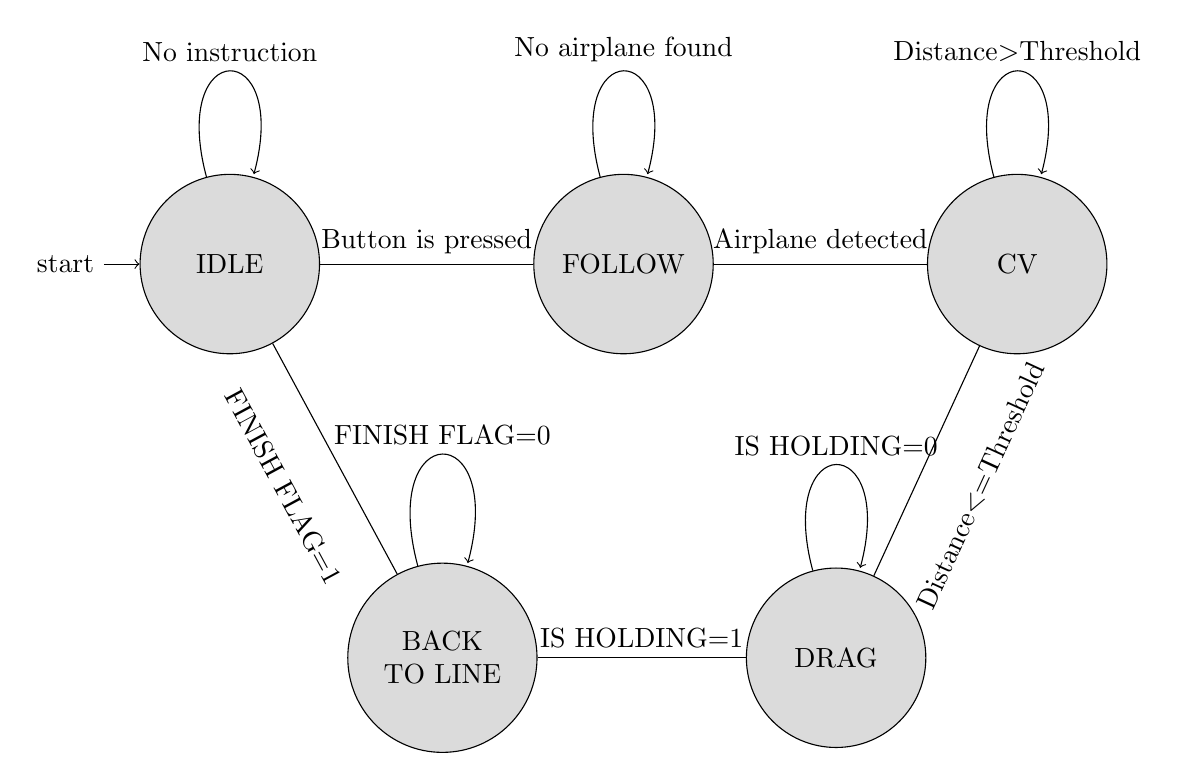
\begin{tikzpicture}
    \tikzstyle{every state}=[fill={rgb:black,1;white,6}, minimum size=1.2cm, text width=2cm, text centered]
    \tikzset{node distance=5cm, auto}
    
    \node[state, initial](q1){IDLE};
    \node[state, right of =q1] (q2) {FOLLOW};
    \node [state, right of=q2](q3) {CV};
    \node [state, below of = q3, xshift=-2.3cm](q4){DRAG};
    \node [state, left of =q4] (q5){BACK TO LINE};
    
    \draw (q1) edge[loop above] node{No instruction} (q1);
    \draw (q1) edge[above] node{Button is pressed} (q2);
    \draw (q2) edge[loop above] node{No airplane found} (q2);
    \draw (q2) edge[above] node{Airplane detected} (q3);
    \draw (q3) edge[loop above] node{Distance$>$Threshold} (q3);
    \draw (q3) edge node[sloped, below=0.5]{Distance$<=$Threshold} (q4);
    \draw (q4) edge[loop above] node{IS HOLDING=0} (q4);
    \draw (q4) edge[above] node{IS HOLDING=1} (q5);
    \draw (q5) edge[loop above] node{FINISH FLAG=0} (q5);
    \draw (q5) edge node[sloped, below=0.5]{FINISH FLAG=1} (q1);
    \end{tikzpicture}
    
    \caption{Operation FSM}
    \label{fig:fsm}
\end{figure}

The FSM above illustrate how our robot works. 
\begin{itemize}
    \item 
    Initially, after running the program, the robot will enter the ``IDLE'' mode. In this case, it will stop moving and wait for coming instructions. The program has a GUI allowing users to start and stop the task by clicking buttons. 
    \item 
    When the Start button is pressed, The robot will enter the ``FOLLOW'' mode to follow the black line that is placed beforehand. During the ``FOLLOW'' mode, the robot will also detect the airplane using \lstinline|detectnet|. 
    \item 
    When the robot successfully see the airplane, it will enter the ``CV'' mode. At this state, the robot will  move towards the light source on the landing gear of the airplane. 
    \item 
    When the distance between the airplane and the robot is close enough, the robot will enter the ``GRAB'' mode, the robot arm and the mechanical claw are activated to hold the handle on the airplane. 
    There are in total 4 sensors on the claw with each's NC (normal-close) terminals connected in series, when anyone of them open, the circuit is open and ``IS HOLDING'' flag will become true, which means that the airplane is successfully dragged. 
    \item 
    When IS HOLDING is true, the robot will enter the ``BACK TO LINE'' state to go back to the line by moving backwards. 
    \item 
    As the line tracker at the back of the robot detect the black line, it will enter the ``HOMING'' state to track the line just like the initial ``FOLLOW'' stage, but in reverse direction. There will be a finish sign in the end of the black line such that all the sensor from the line tracker will detect the black color. 
    
\end{itemize}

In this case, the finish flag becomes true. The whole process is finished after the mechanical claw releases  from the airplane and the state goes back to ``IDLE''.
}
}
\subsection{Arduino}{
Chassis Task:
\begin{figure}[H]
    \tikzstyle{startstop} = [rectangle, rounded corners, minimum width=2.5cm, minimum height=1cm,text centered, draw=black, fill=red!30]
    \tikzstyle{process} = [rectangle, minimum width=2.5cm, minimum height=1cm,text width=2cm, text centered, draw=black, fill=orange!30]
    \tikzstyle{io} = [trapezium, trapezium left angle=70, trapezium right angle=110,text width=2cm, minimum width=1cm, minimum height=1cm, text centered, draw=black, fill=blue!30]
    
    \tikzstyle{decision} = [diamond, minimum width= 0.5cm, minimum height= 0.5cm,text width=2cm, text centered, draw=black, fill=green!30]
    \tikzstyle{arrow} = [thick,->,>=stealth]
    
    \setstretch{1} 
    \begin{tikzpicture}[node distance=3.5cm]
    
    \node (start) [startstop] {start};
    \node (pro1) [process, right of=start] {Setup robot arm command foward};
    \node (pro2) [process, right of =pro1] {Set up sensor feedback foward};
    \node (pro3) [process, right of =pro2] {register chasis cmd};
    \node (pro4) [process, right of =pro3] {initialize chasis};
    \node (pro5) [process, below of =pro4, yshift=0.6cm] {initialize follower};
    \node (de1) [decision, left of =pro5] {switch opmode};
    \node (pro6) [process, left of =de1] {set vx vy wz};
    \node (pro7) [process, below of =pro6, yshift=1.5cm] {follower calc};
    \node (pro8) [process,left of=pro7 ]{set left right};
    \node (pro9) [process, left of =pro8] {send chasis feedback};
    \node (pro10) [process, below of =pro7, yshift=1.5cm] {disable};
    \node  (pro11) [process, below of =pro10,yshift=1.5cm] {sleep 20ms};
    
    \draw [arrow] (start) -- (pro1);
    \draw [arrow] (pro1) -- (pro2);
    \draw [arrow] (pro2) -- (pro3);
    \draw [arrow] (pro3) -- (pro4);
    \draw [arrow] (pro4) -- (pro5);
    \draw [arrow] (pro5) -- (de1);
    \draw [arrow] (de1) -- (pro6);
    \draw [arrow] (de1) |- (pro7);
    \draw [arrow] (de1) |- (pro10);
    \draw [arrow] (pro6) -| (pro9);
    \draw [arrow] (pro7) -- (pro8);
    \draw [arrow] (pro8) -- (pro9);
    \draw [arrow] (pro10) -| (pro9);
    \draw [arrow] (pro9.west) -- ++(-0.5,0) |- (pro11);
    \draw [arrow] (pro11) -| (de1);
    \end{tikzpicture}
\end{figure}
\newpage
Roboarm Task:
\tikzstyle{startstop} = [rectangle, rounded corners, minimum width=2.5cm, minimum height=1cm,text centered, draw=black, fill=red!30]
\tikzstyle{process} = [rectangle, minimum width=2.5cm, minimum height=1cm,text width=2cm, text centered, draw=black, fill=orange!30]
\tikzstyle{io} = [trapezium, trapezium left angle=70, trapezium right angle=110,text width=2cm, minimum width=1cm, minimum height=1cm, text centered, draw=black, fill=blue!30]

\tikzstyle{decision} = [diamond, minimum width= 0.5cm, minimum height= 0.5cm,text width=2cm, text centered, draw=black, fill=green!30]
\tikzstyle{arrow} = [thick,->,>=stealth]

\begin{tikzpicture}[node distance=3.5cm]

\node (start) [startstop] {register roboarm command};
\node (pro1) [process, below of=start, yshift=1cm] {initialise sensors};
\node (de1) [decision, right of=pro1] {sensor OK?};
\node (pro2) [process, right of=de1, yshift=1cm]{red on};
\node (de2) [decision, right of=pro2,yshift=-1cm]{opmode?};
\node (pro3) [process, below of=de2, yshift=0cm]{arm to home};
\node (pro4) [process, left of=pro3]{clamp open};
\node (pro5) [process, below of =pro3, yshift=1cm] {arm to height and angle};
\node (pro6) [process, left of=pro5] {set clamp close or open};
\node (pro7) [process, below of =pro5, yshift=0.6cm] {disable};
\node (pro8) [process, left of=pro6] {send feedback};
\node (pro9) [process, left of=pro8] {sleep 20ms};

\draw [arrow] (start) -- (pro1);
\draw [arrow] (pro1) -- (de1);
\draw [arrow] (de1) -- node{Yes}(pro2);
\draw [arrow] (pro2) -- (de2);
\draw [arrow] (de1) -- node {No}(de2);
\draw [arrow] (de2.east)-- ++(0.5,0) |- (pro3);
\draw [arrow] (de2.east)-- ++(0.5,0) |- (pro5);
\draw [arrow] (de2.east)-- ++(0.5,0) |- (pro7);
\draw [arrow] (pro3) -- (pro4);
\draw [arrow] (pro5) -- (pro6);
\draw [arrow] (pro6) -- (pro8);
\draw [arrow] (pro8) -- (pro9);
\draw [arrow] (pro7) -| (pro8);
\draw [arrow] (pro4) -| (pro8);
\draw [arrow] (pro9) to[bend left=30]  (de2);


\end{tikzpicture}
}


\newpage

\section{Techinical Details}
\subsection{Communication among Jetson and Arduino boards}
We defined our customized protocol as shown in Table \ref{tab:com_protocol}.
\begin{table}[h]
    \centering
    \begin{tabular}{|p{1in}|p{1in}|p{3in}|}
        \hline 
        Offset (Byte) & Length (Byte) & Content \\ \hline 
        0 & 2 & SOF (0x807F) \\ \hline 
        2 & 1 & Packet ID \\ \hline
        3 & 2 & Payload Size \\ \hline
        5 & N & Payload Data \\ \hline
        5+N & 2 & CRC16 \\ \hline 
        7+N & 2 & EOF (0x8080) \\ \hline 
    \end{tabular}
    \caption{Customized data protocol}
    \label{tab:com_protocol}
\end{table}

The pack and send function is demonstrated in pseudocode in Lists below.

\begin{lstlisting}
// Pack and send data to TX 
procedure Send
    buf[0 : 1] = SOF
    buf[2] = id
    buf[3 : 4] = size
    buf[5 : 5+size-1] = data
    crc = crc16(buf[2 : 5+size-1])
    buf[5+size : 6+size] = crc
    buf[7+size : 8+size] = EOF
    send buf to serial
endprocedure 
\end{lstlisting}

\begin{lstlisting}
// Receive data from serial buffer
procedure Receive
    append serial buffer to buf
    sof_idx = -1
    eof_idx = -1
    for i = 0 to eff_len(buf) - 2
        if (buf[i:i+1] == SOF)
            sof_idx = i
        else if (buf[i:i+1] == EOF) 
            unpack buf[sof_idx+2 : eof_idx-1]
        endif
    endfore 
endprocedure 
\end{lstlisting}

\begin{lstlisting}
// unpack data into the respective recv_dst
function unpack (data)
    id = data[0]
    size = data[1 : 2]
    calc_crc = crc16(data[0 : 2+size])
    tran_crc = data[3+size : 4+size]
    if (tran_crc == calc_crc)
        recv_dst[id] = data[3 : 2+size]
        if recv_callback[id] != NULL
            recv_callback[id]()
        endif
    endif
endfunction
\end{lstlisting}

We coded the following function to assign the destination pointer to \lstinline|recv_dst| array: 
\begin{lstlisting}
int communication_register_recv
(communication_t comm, uint8_t pkt_id, void* data_ptr, 
 size_t len, recv_callback_t callback)
\end{lstlisting}

\lstinline|callback| if called if packet of this ID is correctly received. 
In this way, by using the following code
\begin{lstlisting}
void forward_roboarm_cmd() {
    communication_send(&com_S3, ROBOARM_CMD_ID, 
                       &fwd_roboarm_cmd, sizeof(fwd_roboarm_cmd));
}
void forward_sensor_fdbk() {
    communication_send(&com_S2, SENSOR_FDBK_ID, 
                       &fwd_sensor_fdbk, sizeof(fwd_sensor_fdbk));
}
void chassis_setup() {
    communication_register_recv(&com_S2, ROBOARM_CMD_ID, &fwd_roboarm_cmd, 
            sizeof(fwd_roboarm_cmd), (recv_callback_t)&forward_roboarm_cmd);
    communication_register_recv(&com_S3, SENSOR_FDBK_ID, &fwd_sensor_fdbk, 
            sizeof(fwd_sensor_fdbk), (recv_callback_t)&forward_sensor_fdbk);
    ...
\end{lstlisting}
We can easily realize the data switching between the two (or even more, if needed) Arduino boards.
 
% The SOF (start of frame) and EOF (end of frame) 

\subsection{Protocol}
With the communication module above, data can be easily exchanged by sending and receiving the packed structure. There are 4 types of packets: chassis command, chassis feedback, roboarm command, and sensor feedback. 

In Arduino code, they are defined as


\subsection{DC Motor speed control with PID}

To measure the wheel speed, following macro function is coded to assign the motor and register encoder interrupt.
\begin{lstlisting}
#define MOTOR_ASSIGN(NAME, PIN_1, PIN_2, PIN_PWM, PIN_A, PIN_B)     \
void isr_##NAME();                                                  \
struct motor_device NAME = {                                        \
    .pin_1 = PIN_1, .pin_2 = PIN_2, .pin_pwm = PIN_PWM,             \
    .pin_ecd_A = PIN_A, .pin_ecd_B = PIN_B, .ecd_isr = isr_##NAME   \
};                                                                  \
void isr_##NAME(void) {                                             \
    if(digitalRead(NAME.pin_ecd_B)) NAME.data.total_ecd++;          \
    else NAME.data.total_ecd--;                                     \
}
\end{lstlisting}

PID library developed by DJI Robomaster is borrowed 
and applied to control the motors, with the four speed of mecanum as reference
and encoder measured speed as feedback. The speed unit is is in RPM, and PID parameters used are
\begin{table}[H]
    \centering
    \begin{tabular}{|p{2in}|p{2in}|}
       \hline 
       Parameter  & Value  \\ \hline 
       $k_p$  & 0.8 \\ \hline 
       $k_i$ & 0.1 \\ \hline 
       $k_d$ & 0 \\ \hline 
       Maximum input error & 0 \\ \hline 
       Maximum output & MOTOR\_DUTY\_MAX (255) \\ \hline 
       Integral limit & MOTOR\_DUTY\_MAX / 5 (51) \\ \hline
    \end{tabular}
    \caption{Chassis wheel motor PID params}
    \label{tab:chassis_pid_params}
\end{table}

\subsection{Line following}
The raw line tracker value is stored in a 8-bit variable as
\begin{lstlisting}
value = (digitalRead(sensor->pin_3) << 3) |
        (digitalRead(sensor->pin_2) << 2) |
        (digitalRead(sensor->pin_1) << 1) |
        (digitalRead(sensor->pin_0));
\end{lstlisting}

And an error is calculated based this value, if the two outer sensors see black, 
then use the outer sensor's bias, otherwise, use the two inner sensors.  
\begin{lstlisting}
error = (((value & 0b1000) >> 3) - ((value & 0b0001))) * 3;
if (error == 0)
   error = ((value & 0b0100) >> 2) - ((value & 0b0010) >> 1);
\end{lstlisting}

Use this error as feedback, a PID controller is applied. The reference is always 0, and output is used to get the left and right side wheel speed as 
\begin{lstlisting}
left = 1 - pid_out;
right = 1 + pid_out;
\end{lstlisting}

\subsection{Roboarm Calculate}
For our 2-DoF roboarm, Joint-1 controls the backward-forward of the arm, which also change the height of the Joint-2. Joint-2 controls the pitch angle of the clamp. Thus the roboarm can be controlled via a height and an angle.

Upon receiving the height, the angle $\theta$ of Join-1 servo is computed by 
\begin{lstlisting}
h = height - H_OFFSET;
if (h > ARM_LEN)
    h = ARM_LEN;
theta = degrees( acos(h / (ARM_LEN + 0.1)) );
\end{lstlisting}

\subsection{Clamp close}
When the ``close'' flag in roboarm command is 1, the clamp will close. It will first close util the 
micro switch assert, and then close for a further 20 degrees to make the grabbing tight enough.
This is implemented with the help of ``clamp\_tight'' flag. Each loop it will do
\begin{lstlisting}
if switch touched
    clamp_deg = clamp_deg - 1
    servo.set_angle(clamp_deg)
    clamp_tight = false
else if clamp_tight == false
    clamp_deg = clamp_deg - 20
    servo.set_angle(clamp_deg)
    clamp_tight = true
endif
\end{lstlisting}
\newpage 

\section{Reflection}{

When we are developing our robot, we met several challenges or difficulties. This section will talk about difficulties and our solutions.

\subsection{Problem with DetectNet}{
We mentioned that Computer Vision techniques are adopted to recognize the airplane. However, the process of detecting the airplane is not successful initially due to mainly two factors: 
\begin{enumerate}
    \item 
    Our airplane, especially installed with a handle and a light source, is sometimes not similar to the training dataset of the Detectnet. 
    \item
    There may be some interference (i,e., human, chairs) when testing that avoid the model from recognizing the object. 
\end{enumerate}

To address the problem, We firstly tried to train our own model with our custom pictures as the training dataset. However, we met several issues such as the version incompatibility of Numpy and Pytorch on Jetson Nano. As a result, although we successfully have the training data, we eventually failed to finish validation and obtain a valid model.

Instead of changing the model, we shift our focus to alter the environment to better fit the original training data from DetectNet. 
We found that CV actually works well when the airplane is around 1 meter apart from the camera, and thus we will always follow this standard when making the black line and placing the airplane.
% During the tasting of Detectnet, we also found that the bounding box of the model to the airplane aren't stable on many occations. 

In order to remove any probable disturbances, we will also find places with no people appear in the camera. Finally, we observed that it is more easier if the airplane is placed at some angle between the camera. It seems that the confidence rate is expected to increase with the visibility of propeller and the body of the airplane.


}

\subsection{Problem with dragging}{
After the model locates the airplane, the robot is expected to move towards the robot through light seeker as demonstrated in the required function. The process of dragging after the light seeking is initially difficult to solve because of several challenges: 
\begin{enumerate}
    \item 
    The robots arm's servo motors' torque are too low and it is difficult to control the angle of mechanical claw to the ground. The mechanical claw is initially not able to rose to a certain degree as we wrote in the program. This overload phenomenon may destroy the servo motor and even the servos.
    \item 
    The four sensor installed on the mechanical claw are sometime not sensitive enough, but the mechanical claw may fail to hold the airplane tightly if the sensors are too sensitive.
\end{enumerate}
To mitigate the first problem, we added rubber band from robot arm and the Jetson nano board to decrease the load of the servo motor. We also used other things like ties and tape to strengthen the ability of robot arm to hold the heavy objects. In addition, the servo motors are rated to operate at 4.8-6.0V, so we bought a seperated Buck converter to provide around 5.5V voltage to the roboarm servos to make their torque higher than the one with USB powered.

The second problems are relatively harder to solve, because it is time consuming to adjust the distance of various parameters. To achieve our aims, we fix the position of the sensors, make the handle become thicker, and increase the angle of the mechanical claw to better clamp the airplane.  

}
\subsection{Problems with Serial communication}
    The Serial port socket on the Arduino extension board is too lose, and the transmission corrupts from time to time. We applied CRC16 checksum in protocol to eliminate dirty commands which could be dangerous, but timeout from time to time due to bad connections cannot be easily solved.
    % With our original receive function, when one corrupted,  
}

\subsection{Problems with I2C communication with sensors}
The 
% fucking retard 
bread board never works. The holes are so 
% damn 
lose and the I2C communication is interrupted by it from time to time. When request data from I2C bus, 
if the connection is interrupted, the Arduino will wait forever for the data that should have arrived. As a result the program hangs at the I2C read operation and the car dies. 

We identified the 
% fucking 
problem too late and did not have enough time to make a PCB or solder the Y-lines to share the I2C bus 
robustly. As a result, in order to at least show you something and avoid a zero-mark in demo, we removed the INA226 and MPU6050 sensors both physically and in program, and connected the BMP and ToF directly to the extension board's two I2C ports to avoid using bread board. % Damn.
% It is appreciated if 

% \section{Conclusion}{
In this project, we developed an autonomous towing tractor for model plane airfields. 

}
% \begin{figure}[H]
    \tikzstyle{startstop} = [rectangle, rounded corners, minimum width=2.5cm, minimum height=1cm,text centered, draw=black, fill=red!30]
    \tikzstyle{process} = [rectangle, minimum width=2.5cm, minimum height=1cm,text width=2cm, text centered, draw=black, fill=orange!30]
    \tikzstyle{io} = [trapezium, trapezium left angle=70, trapezium right angle=110,text width=2cm, minimum width=1cm, minimum height=1cm, text centered, draw=black, fill=blue!30]
    
    \tikzstyle{decision} = [diamond, minimum width= 0.5cm, minimum height= 0.5cm,text width=2cm, text centered, draw=black, fill=green!30]
    \tikzstyle{arrow} = [thick,->,>=stealth]
    
    \setstretch{1} 
    \begin{tikzpicture}[node distance=3.5cm]
    
    \node (start) [startstop] {start};
    \node (pro1) [process, right of=start] {Setup robot arm command foward};
    \node (pro2) [process, right of =pro1] {Set up sensor feedback foward};
    \node (pro3) [process, right of =pro2] {register chasis cmd};
    \node (pro4) [process, right of =pro3] {initialize chasis};
    \node (pro5) [process, below of =pro4, yshift=0.6cm] {initialize follower};
    \node (de1) [decision, left of =pro5] {switch opmode};
    \node (pro6) [process, left of =de1] {set vx vy wz};
    \node (pro7) [process, below of =pro6, yshift=1.5cm] {follower calc};
    \node (pro8) [process,left of=pro7 ]{set left right};
    \node (pro9) [process, left of =pro8] {send chasis feedback};
    \node (pro10) [process, below of =pro7, yshift=1.5cm] {disable};
    \node  (pro11) [process, below of =pro10,yshift=1.5cm] {sleep 20ms};
    
    \draw [arrow] (start) -- (pro1);
    \draw [arrow] (pro1) -- (pro2);
    \draw [arrow] (pro2) -- (pro3);
    \draw [arrow] (pro3) -- (pro4);
    \draw [arrow] (pro4) -- (pro5);
    \draw [arrow] (pro5) -- (de1);
    \draw [arrow] (de1) -- (pro6);
    \draw [arrow] (de1) |- (pro7);
    \draw [arrow] (de1) |- (pro10);
    \draw [arrow] (pro6) -| (pro9);
    \draw [arrow] (pro7) -- (pro8);
    \draw [arrow] (pro8) -- (pro9);
    \draw [arrow] (pro10) -| (pro9);
    \draw [arrow] (pro9.west) -- ++(-0.5,0) |- (pro11);
    \draw [arrow] (pro11) -| (de1);
    \end{tikzpicture}
\end{figure}
% \tikzstyle{startstop} = [rectangle, rounded corners, minimum width=2.5cm, minimum height=1cm,text centered, draw=black, fill=red!30]
\tikzstyle{process} = [rectangle, minimum width=2.5cm, minimum height=1cm,text width=2cm, text centered, draw=black, fill=orange!30]
\tikzstyle{io} = [trapezium, trapezium left angle=70, trapezium right angle=110,text width=2cm, minimum width=1cm, minimum height=1cm, text centered, draw=black, fill=blue!30]

\tikzstyle{decision} = [diamond, minimum width= 0.5cm, minimum height= 0.5cm,text width=2cm, text centered, draw=black, fill=green!30]
\tikzstyle{arrow} = [thick,->,>=stealth]

\begin{tikzpicture}[node distance=3.5cm]

\node (start) [startstop] {register roboarm command};
\node (pro1) [process, below of=start, yshift=1cm] {initialise sensors};
\node (de1) [decision, right of=pro1] {sensor OK?};
\node (pro2) [process, right of=de1, yshift=1cm]{red on};
\node (de2) [decision, right of=pro2,yshift=-1cm]{opmode?};
\node (pro3) [process, below of=de2, yshift=0cm]{arm to home};
\node (pro4) [process, left of=pro3]{clamp open};
\node (pro5) [process, below of =pro3, yshift=1cm] {arm to height and angle};
\node (pro6) [process, left of=pro5] {set clamp close or open};
\node (pro7) [process, below of =pro5, yshift=0.6cm] {disable};
\node (pro8) [process, left of=pro6] {send feedback};
\node (pro9) [process, left of=pro8] {sleep 20ms};

\draw [arrow] (start) -- (pro1);
\draw [arrow] (pro1) -- (de1);
\draw [arrow] (de1) -- node{Yes}(pro2);
\draw [arrow] (pro2) -- (de2);
\draw [arrow] (de1) -- node {No}(de2);
\draw [arrow] (de2.east)-- ++(0.5,0) |- (pro3);
\draw [arrow] (de2.east)-- ++(0.5,0) |- (pro5);
\draw [arrow] (de2.east)-- ++(0.5,0) |- (pro7);
\draw [arrow] (pro3) -- (pro4);
\draw [arrow] (pro5) -- (pro6);
\draw [arrow] (pro6) -- (pro8);
\draw [arrow] (pro8) -- (pro9);
\draw [arrow] (pro7) -| (pro8);
\draw [arrow] (pro4) -| (pro8);
\draw [arrow] (pro9) to[bend left=30]  (de2);


\end{tikzpicture}

\end{document}
